\chapter{Results}

\section{Term Statistics}

\begin{figure}[h]
    \centering
    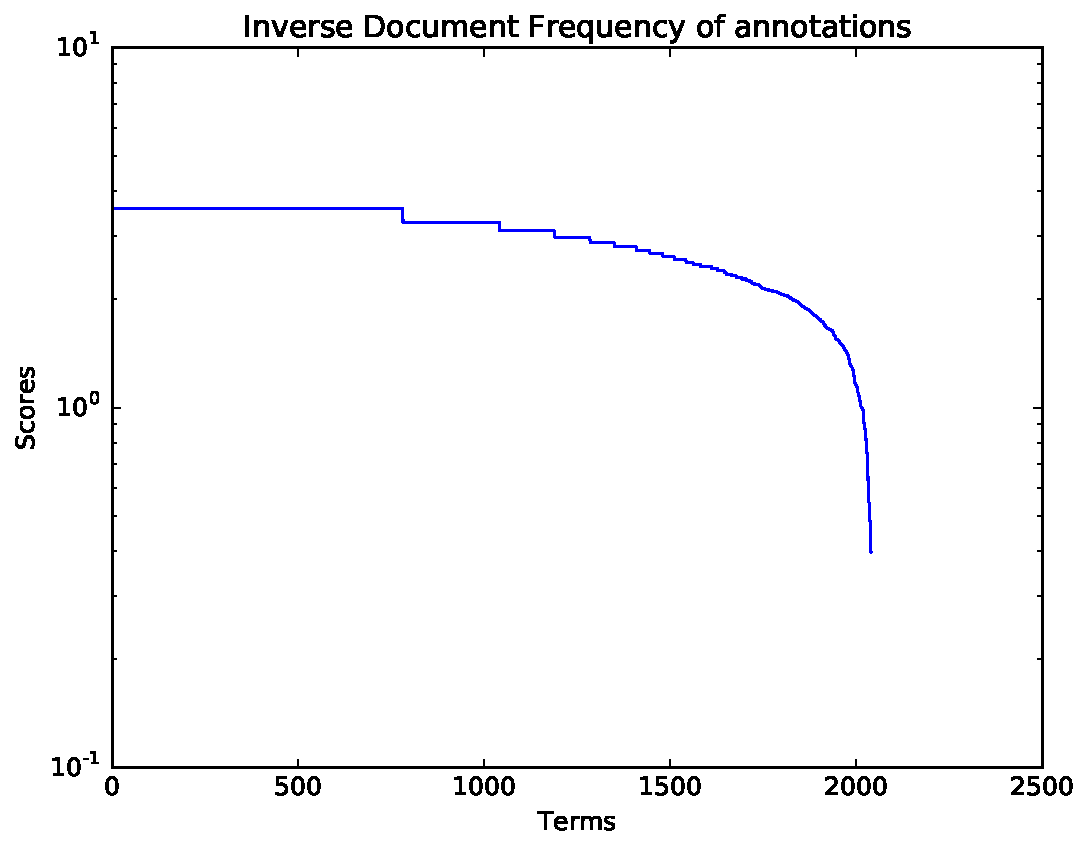
\includegraphics[width=0.7\textwidth]{graphs/idf-scores}
    \caption{IDF scores for terms in the annotations}
    \label{fig:idf-scores}
\end{figure}

Concepts chosen for relevance assessment ad hears to Zipf's law. The graph in Figure \ref{fig:idf-scores} illustrates the IDF scores for each of the concepts in the corpus of annotations. Just 40 concepts are shown out of a total of 2041. 

Note that the notion of concepts are different to terms since a concept can contain more than once word (this is possible through tags, where a tag can contain multiple words such as `shopping mall' and `street sign').

\FloatBarrier
\section{Annotation Statistics}

In total, five annotators managed to annotate a total of \todo{10,982} images across all annotation methodologies. Figure \ref{fig:annotator-breakdown} illustrates the number of annotations completed by each annotator. Two annotators accounted for the majority of the annotations, while three others provide an additional \todo{904}. The exact number of each annotation type, the total time it took to annotate each annotation type and the average time it took to annotate is shown in Table \ref{table:annotation-stats}.

\begin{figure}[!htb]
    \centering
    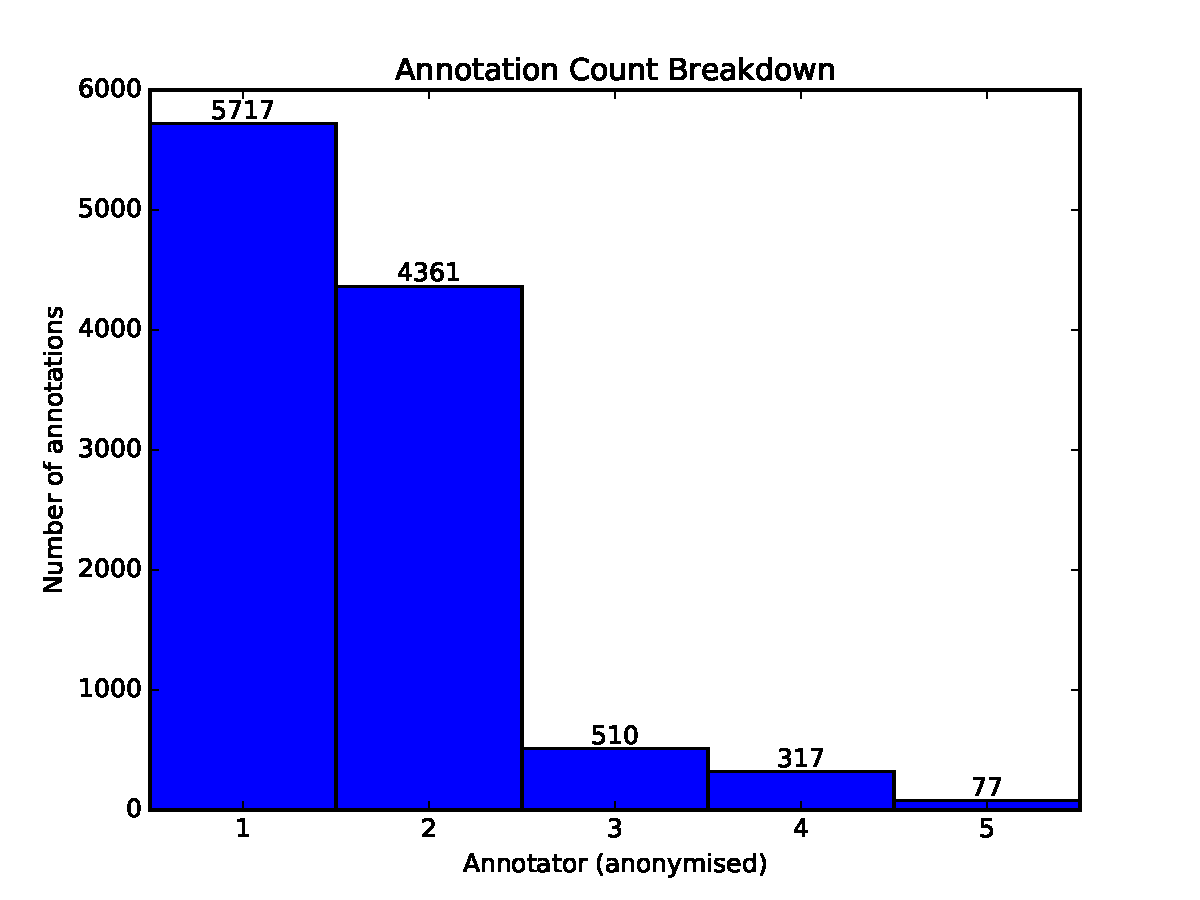
\includegraphics[width=0.95\textwidth]{graphs/annotator-breakdown}
    \caption{Total number of annotations by annotator}
    \label{fig:annotator-breakdown}
\end{figure}

\begin{table}[!htb]
    \centering
    \begin{tabular}{ | l | l | l | l | p{5cm} |}
    \hline
    Name & Count & Average Time & Total Time \\ \hline
    Text & 3172 & 1 minute & 2 days, 23 hours \\ \hline
    Tag & 2897 & 31 seconds & 23 hours, 40 minutes \\ \hline
    Query & 3616 & 16 seconds & 15 hours, 10 minutes \\ \hline
    Assessment & 1327 & 58 seconds & 21 hours, 36 minutes \\ \hline
    \end{tabular}
    \caption{Annotation Statistics}
    \label{table:annotation-stats}
\end{table}

Textual annotations accounted for the most amount of time in the collection process by far. The most number of annotations collected for a methodology were the query annotations. Accounts from annotators noted that the relevance assessments were the most difficult to collect. 

\FloatBarrier
\section{Retrieval Effectiveness}

Each experiment is displayed as a table which provides the results from \verb|trec_eval| and as a precision-recall graph. The results from only the manually annotated images are displayed first. Tables \ref{table:manual-text},  \ref{table:manual-tag}, \ref{table:manual-query}, \ref{table:manual-assessment} display the \verb|trec_eval| results, and the same results but performing search on all of the annotations types in Table \ref{table:manual-all}. These results are visualised as a precision-recall graph in Figure \ref{fig:manual-result}.

\begin{table}[htb]
    \parbox{.45\linewidth}{
    \begin{tabular}{ | l | l | }
    \hline
    Metric & Score \\ \hline
	num\_q & 48 \\ \hline
	num\_ret & 27382 \\ \hline
	num\_rel & 6708 \\ \hline
	num\_rel\_ret & 1062 \\ \hline
	map & 0.5436 \\ \hline
	gm\_map & 0.3442 \\ \hline
	Rprec & 0.5506 \\ \hline
	bpref & 0.5564 \\ \hline
	recip\_rank & 0.9223 \\ \hline
	iprec\_at\_recall\_0.00 & 0.9596 \\ \hline
	iprec\_at\_recall\_0.10 & 0.8213 \\ \hline
	iprec\_at\_recall\_0.20 & 0.6831 \\ \hline
	iprec\_at\_recall\_0.30 & 0.5999 \\ \hline
	iprec\_at\_recall\_0.40 & 0.5567 \\ \hline
	iprec\_at\_recall\_0.50 & 0.5296 \\ \hline
	iprec\_at\_recall\_0.60 & 0.5236 \\ \hline
	iprec\_at\_recall\_0.70 & 0.4827 \\ \hline
	iprec\_at\_recall\_0.80 & 0.3974 \\ \hline
	iprec\_at\_recall\_0.90 & 0.2895 \\ \hline
	iprec\_at\_recall\_1.00 & 0.2458 \\ \hline
	P\_5 & 0.8833 \\ \hline
	P\_10 & 0.8333 \\ \hline
	P\_15 & 0.7778 \\ \hline
	P\_20 & 0.7365 \\ \hline
	P\_30 & 0.6437 \\ \hline
	P\_100 & 0.2150 \\ \hline
	P\_200 & 0.1083 \\ \hline
	P\_500 & 0.0434 \\ \hline
	P\_1000 & 0.0221 \\ \hline
    \end{tabular}
    \caption{Text}
    \label{table:manual-text}
    }
    \hfill
    \parbox{.45\linewidth}{
    \begin{tabular}{ | l | l | }
    \hline
    Metric & Score \\ \hline
	num\_q & 48 \\ \hline
	num\_ret & 2850 \\ \hline
	num\_rel & 6708 \\ \hline
	num\_rel\_ret & 1040 \\ \hline
	map & 0.5468 \\ \hline
	gm\_map & 0.3540 \\ \hline
	Rprec & 0.5493 \\ \hline
	bpref & 0.5865 \\ \hline
	recip\_rank & 0.9578 \\ \hline
	iprec\_at\_recall\_0.00 & 0.9735 \\ \hline
	iprec\_at\_recall\_0.10 & 0.8409 \\ \hline
	iprec\_at\_recall\_0.20 & 0.6636 \\ \hline
	iprec\_at\_recall\_0.30 & 0.5884 \\ \hline
	iprec\_at\_recall\_0.40 & 0.5441 \\ \hline
	iprec\_at\_recall\_0.50 & 0.5112 \\ \hline
	iprec\_at\_recall\_0.60 & 0.5016 \\ \hline
	iprec\_at\_recall\_0.70 & 0.4751 \\ \hline
	iprec\_at\_recall\_0.80 & 0.4540 \\ \hline
	iprec\_at\_recall\_0.90 & 0.3674 \\ \hline
	iprec\_at\_recall\_1.00 & 0.2521 \\ \hline
	P\_5 & 0.9000 \\ \hline
	P\_10 & 0.8396 \\ \hline
	P\_15 & 0.7972 \\ \hline
	P\_20 & 0.7469 \\ \hline
	P\_30 & 0.6514 \\ \hline
	P\_100 & 0.2158 \\ \hline
	P\_200 & 0.1083 \\ \hline
	P\_500 & 0.0433 \\ \hline
	P\_1000 & 0.0217 \\ \hline
    \end{tabular}
    \caption{Tag}
    \label{table:manual-tag}
    }
\end{table}

% query
% trec_eval results

\begin{table}[htb]
    \parbox{.45\linewidth}{
    \begin{tabular}{ | l | l | }
    \hline
    Metric & Score \\ \hline
	num\_q & 48 \\ \hline
	num\_ret & 9353 \\ \hline
	num\_rel & 6708 \\ \hline
	num\_rel\_ret & 1559 \\ \hline
	map & 0.6400 \\ \hline
	gm\_map & 0.4809 \\ \hline
	Rprec & 0.6428 \\ \hline
	bpref & 0.6531 \\ \hline
	recip\_rank & 0.9653 \\ \hline
	iprec\_at\_recall\_0.00 & 0.9924 \\ \hline
	iprec\_at\_recall\_0.10 & 0.9317 \\ \hline
	iprec\_at\_recall\_0.20 & 0.8617 \\ \hline
	iprec\_at\_recall\_0.30 & 0.7472 \\ \hline
	iprec\_at\_recall\_0.40 & 0.6434 \\ \hline
	iprec\_at\_recall\_0.50 & 0.6177 \\ \hline
	iprec\_at\_recall\_0.60 & 0.5445 \\ \hline
	iprec\_at\_recall\_0.70 & 0.5077 \\ \hline
	iprec\_at\_recall\_0.80 & 0.4859 \\ \hline
	iprec\_at\_recall\_0.90 & 0.4062 \\ \hline
	iprec\_at\_recall\_1.00 & 0.3854 \\ \hline
	P\_5 & 0.9292 \\ \hline
	P\_10 & 0.8750 \\ \hline
	P\_15 & 0.8250 \\ \hline
	P\_20 & 0.7781 \\ \hline
	P\_30 & 0.7090 \\ \hline
	P\_100 & 0.3000 \\ \hline
	P\_200 & 0.1613 \\ \hline
	P\_500 & 0.0648 \\ \hline
	P\_1000 & 0.0325 \\ \hline
    \end{tabular}
    \caption{Query}
    \label{table:manual-query}
    }
    \parbox{.45\linewidth}{
    \begin{tabular}{ | l | l | }
    \hline
    Metric & Score \\ \hline
	num\_q & 36 \\ \hline
	num\_ret & 2323 \\ \hline
	num\_rel & 5009 \\ \hline
	num\_rel\_ret & 695 \\ \hline
	map & 0.5649 \\ \hline
	gm\_map & 0.3587 \\ \hline
	Rprec & 0.5536 \\ \hline
	bpref & 0.5784 \\ \hline
	recip\_rank & 0.9504 \\ \hline
	iprec\_at\_recall\_0.00 & 0.9661 \\ \hline
	iprec\_at\_recall\_0.10 & 0.8252 \\ \hline
	iprec\_at\_recall\_0.20 & 0.7426 \\ \hline
	iprec\_at\_recall\_0.30 & 0.6181 \\ \hline
	iprec\_at\_recall\_0.40 & 0.5903 \\ \hline
	iprec\_at\_recall\_0.50 & 0.5852 \\ \hline
	iprec\_at\_recall\_0.60 & 0.5521 \\ \hline
	iprec\_at\_recall\_0.70 & 0.5036 \\ \hline
	iprec\_at\_recall\_0.80 & 0.4212 \\ \hline
	iprec\_at\_recall\_0.90 & 0.3263 \\ \hline
	iprec\_at\_recall\_1.00 & 0.1833 \\ \hline
	P\_5 & 0.8722 \\ \hline
	P\_10 & 0.8194 \\ \hline
	P\_15 & 0.7630 \\ \hline
	P\_20 & 0.6875 \\ \hline
	P\_30 & 0.5593 \\ \hline
	P\_100 & 0.1931 \\ \hline
	P\_200 & 0.0965 \\ \hline
	P\_500 & 0.0386 \\ \hline
	P\_1000 & 0.0193 \\ \hline
    \end{tabular}
    \caption{Relevance Assessment}
    \label{table:manual-assessment}
    }
\end{table}

\begin{table}[htb]
    \centering
    \begin{tabular}{ | l | l | }
    \hline
    Metric & Score \\ \hline
    num\_q & 48 \\ \hline
    num\_ret & 9353 \\ \hline
    num\_rel & 6708 \\ \hline
    num\_rel\_ret & 1559 \\ \hline
    map & 0.6400 \\ \hline
    gm\_map & 0.4809 \\ \hline
    Rprec & 0.6428 \\ \hline
    bpref & 0.6531 \\ \hline
    recip\_rank & 0.9653 \\ \hline
    iprec\_at\_recall\_0.00 & 0.9924 \\ \hline
    iprec\_at\_recall\_0.10 & 0.9317 \\ \hline
    iprec\_at\_recall\_0.20 & 0.8617 \\ \hline
    iprec\_at\_recall\_0.30 & 0.7472 \\ \hline
    iprec\_at\_recall\_0.40 & 0.6434 \\ \hline
    iprec\_at\_recall\_0.50 & 0.6177 \\ \hline
    iprec\_at\_recall\_0.60 & 0.5445 \\ \hline
    iprec\_at\_recall\_0.70 & 0.5077 \\ \hline
    iprec\_at\_recall\_0.80 & 0.4859 \\ \hline
    iprec\_at\_recall\_0.90 & 0.4062 \\ \hline
    iprec\_at\_recall\_1.00 & 0.3854 \\ \hline
    P\_5 & 0.9292 \\ \hline
    P\_10 & 0.8750 \\ \hline
    P\_15 & 0.8250 \\ \hline
    P\_20 & 0.7781 \\ \hline
    P\_30 & 0.7090 \\ \hline
    P\_100 & 0.3000 \\ \hline
    P\_200 & 0.1613 \\ \hline
    P\_500 & 0.0648 \\ \hline
    P\_1000 & 0.0325 \\ \hline
    \end{tabular}
    \caption{All manual annotations}
    \label{table:manual-all}
\end{table}

\begin{figure}[htb]
    \centering
    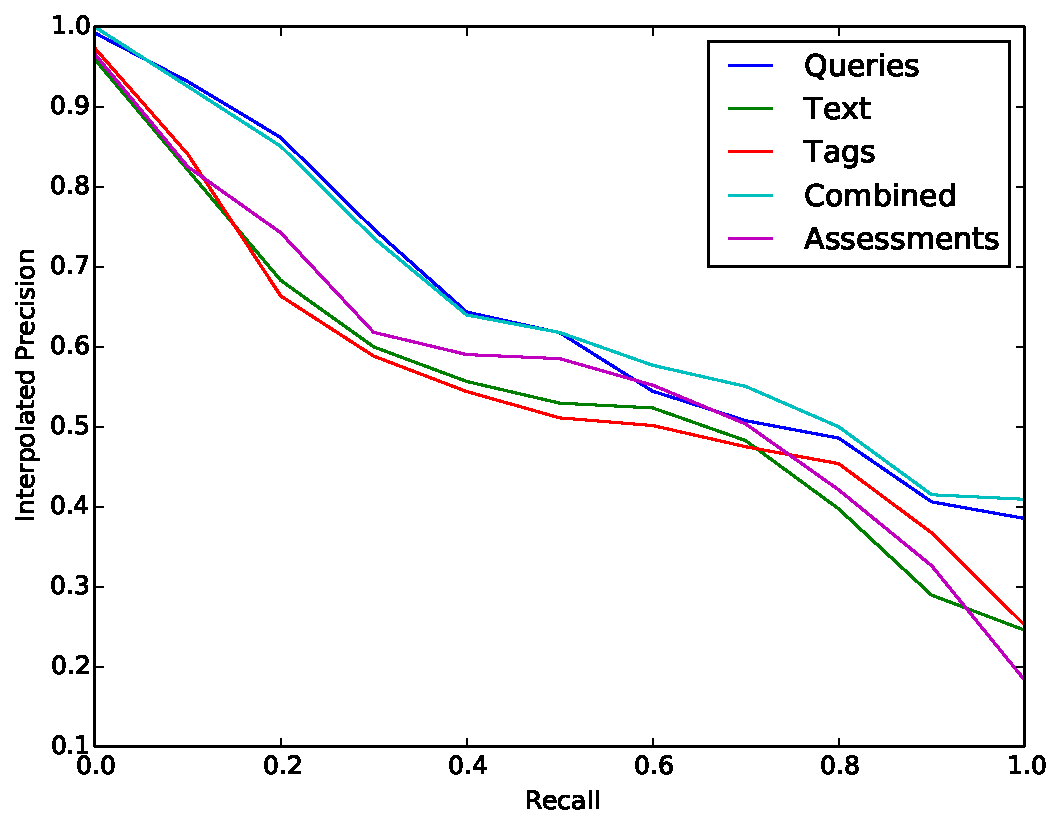
\includegraphics[width=0.95\textwidth]{graphs/manual-result}
    \caption{Precision-recall curves for the manual annotations}
    \label{fig:manual-result}
\end{figure}

\FloatBarrier

A neural network was trained on the manual textual, tag, and query annotations. The network was able to produce captions for every image in the collection. The automatic captions that were generated were then evaluated in the same way as the manual annotations. 

\begin{table}[h]
    \centering
    \begin{tabular}{|c|c|c|c|}
        \hline
         Methodology & MAP & RR & P@10 \\ \hline
         Text & 0.0048 & 0.0248 & 0.0196 \\ \hline
         Tag & 0.0083 & 0.0184 & 0.022  \\ \hline
         Query & 0.0076 & 0.0174 & 0.0021 \\ \hline
         All & 0.0164 & 0.0393 & 0.0169 \\ \hline
    \end{tabular}
    \caption{MAP, Reciprocal Rank, and Precision at 10 scores for the learnt annotations}
    \label{table:learnt-results}
\end{table}

\begin{figure}[h]
    \centering
    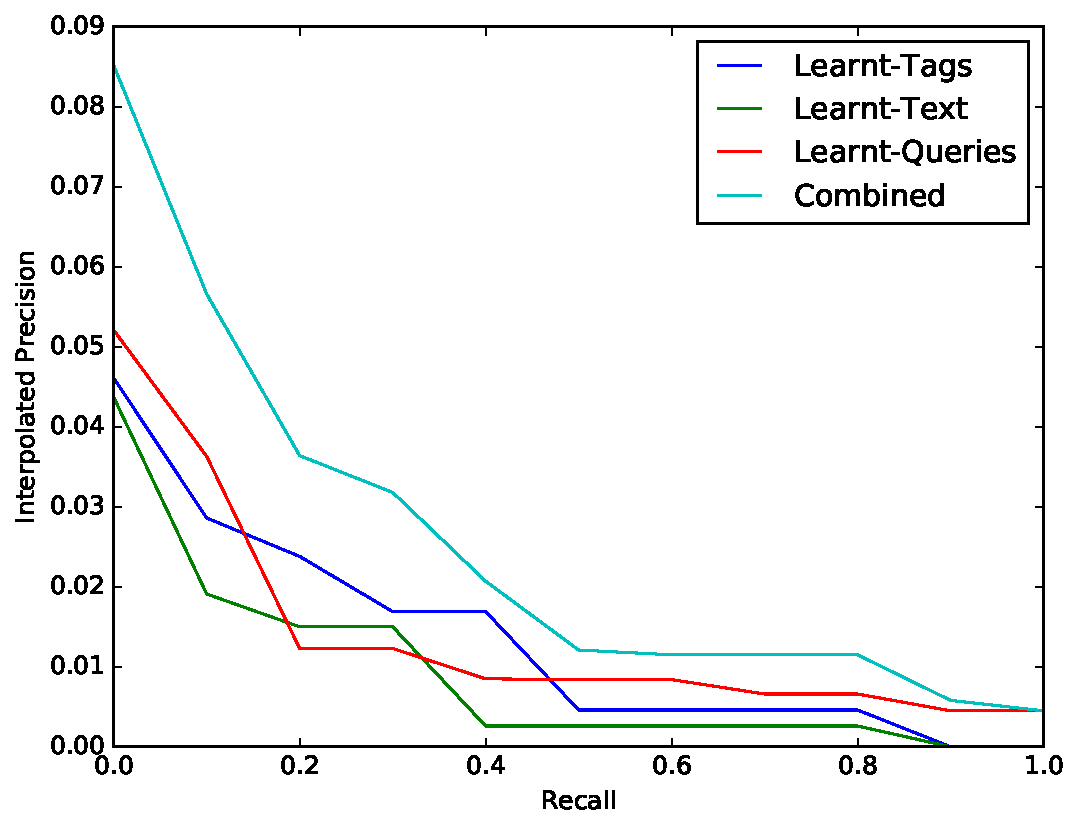
\includegraphics[width=0.95\textwidth]{graphs/learnt-result}
    \caption{Precision-recall curves for the learnt annotations}
    \label{fig:manual-result}
\end{figure}

There is no clear individual annotation methodology that outperforms the others, the scores are too low to indicate this. Combining the three automatic annotations together, however, does seem to increase the overall precision.

\FloatBarrier
The number of iterations the neural network covered for each annotation methodology is visualised in Figures \ref{fig:val-loss-1} and \ref{fig:val-loss-2}. The results of the automatic captioning do not get better over time --- in fact they get worse.

\begin{figure}[h]
    \centering
    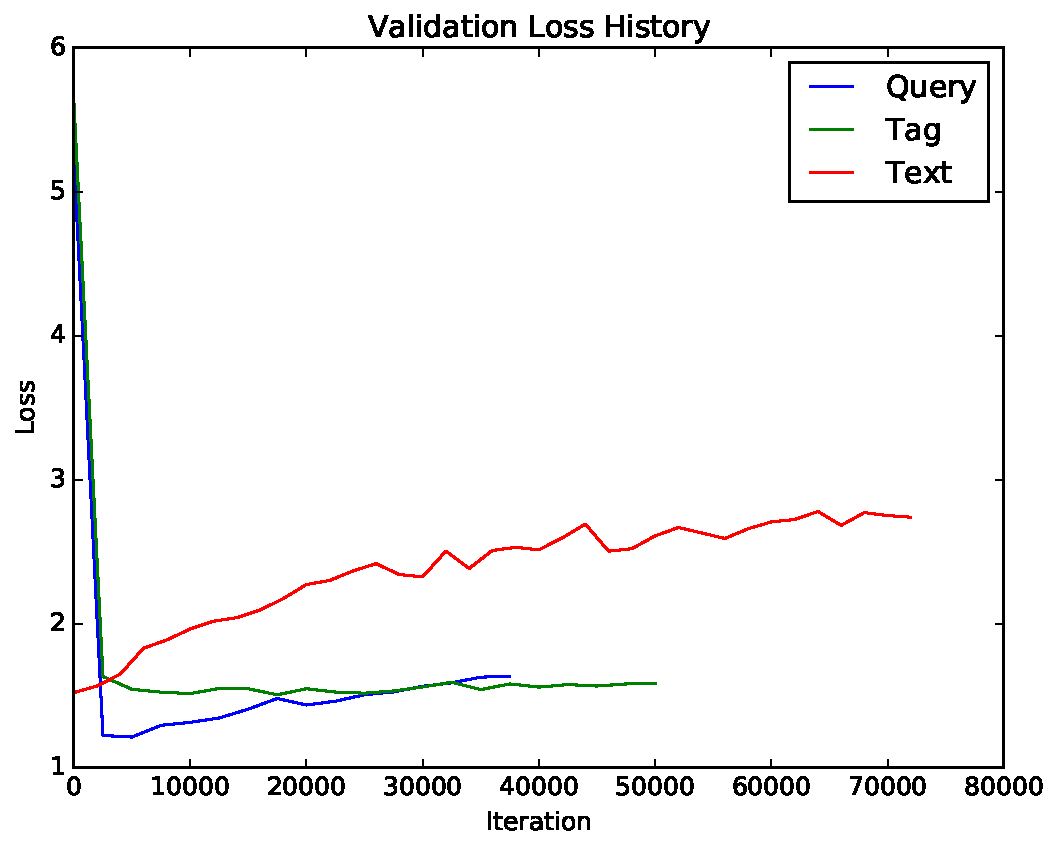
\includegraphics[width=0.95\textwidth]{graphs/initial-validation-loss-history}
    \caption{Validation loss history (\textless 100,000 iterations)}
    \label{fig:val-loss-1}
\end{figure}

\begin{figure}[h]
    \centering
    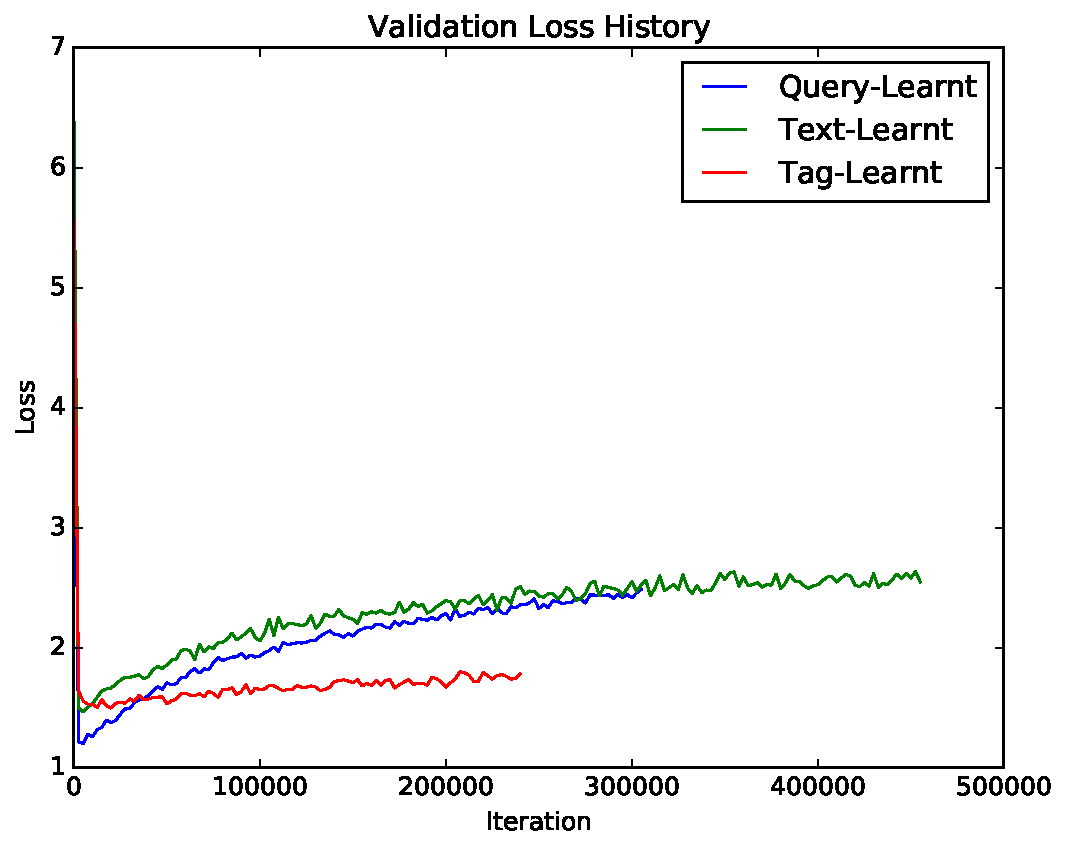
\includegraphics[width=0.95\textwidth]{graphs/validation-loss-history}
    \caption{Validation loss history (\textgreater 200,000 iterations)}
    \label{fig:val-loss-2}
\end{figure}